\documentclass{ExamJHSEngl}
% ExamJHSEngl v0.5.2

\showAnswer{0}

\begin{document}

\chapter[2023]{
	\hspace*{-0.3em}
	\headLine{2023}{年包头市第一次区域联考学业水平测试}{英语}{}
}


\section{\Choices{70}}

\subsection{听力(共2节,20分)}
\Directions{听录音,根据各题要求选择最佳答案,并将答题卡上对应题目的答案标号涂黑。每项内容读两遍。}

\subsubsection{\Scores{5}{1}}
\Directions{听下面5段对话,选出与录音内容相一致的图片。}

\begin{figure}[htp]
  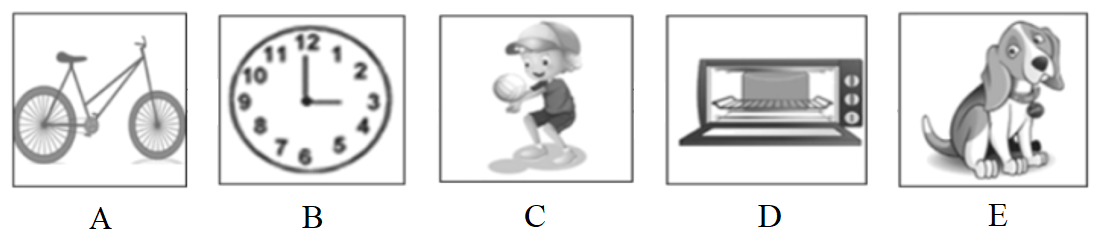
\includegraphics[height=6em]{figures/example-1.png}
  
  \completion[1.5]{A}
  \completion[1.5]{E}
  \completion[1.5]{C}
  \completion[1.5]{D}
  \completion[1.5]{B}
\end{figure}


\subsubsection{\Scores{15}{1}}
\Directions{听下面5段对话或独白。每段对话或独白后有几个小题,从题中所给的A、B、C三个选项中选出最佳选项。}

\Directions{听材料,回答问题。}

\begin{enumerate}[start=6,ref={\arabic*},labelsep=-0.1em,itemsep=0em]

  \item[\choice{A}] What is Li Na good at?
  \option{The violin.}{The piano.}{The guitar. }
  
  \item[\choice{C}] How old is Li Na? 
  \option{Five.}{Seven.}{Twelve.}
  
  \item[\choice{B}] What does the girl think of Li Na?
  \option{She's friendly.}{She's hardworking.}{She's humorous.}

\end{enumerate}

\Directions{听材料,回答问题。}

\begin{enumerate}[resume,ref={\arabic*},labelsep=-0.1em,itemsep=0em]

  \item[\choice{C}] What is Jackson's problem with learning French?
  \option{Learning grammar rules.}{Remembering new words.}{Understanding native speakers.}
  
  \item[\choice{B}] How does Jackson learn French?
  \option{By listening to tapes, classmates.}{By attending classes.}{By talking with his}
  
   
  \item[\choice{A}] What does the woman advise Jackson to do?
  \option{To use French often.}{To try different books.}{To watch TV programs. }

\end{enumerate}

\Directions{听材料,回答问题。}

\begin{enumerate}[resume,ref={\arabic*},labelsep=-0.1em,itemsep=0em]

  \item[\choice{B}] How did the boy feel at first?
  \option{Sad.}{Nervous.}{Relaxed. }
  
  \item[\choice{A}] What exam will be difficult according to some students?
  \option{Math.}{English.}{Geography. }
  
  \item[\choice{A}] What does Anna advise the boy to do?
  \option{To study hard.}{To ask teachers for help.}{To listen to others. }
 
\end{enumerate}

\Directions{听材料,回答问题。}

\begin{enumerate}[resume,ref={\arabic*},labelsep=-0.1em,itemsep=0em]

  \item[\choice{C}] What time is it now?
  \option{5:12 pm.}{2:50 pm.}{2:15 pm. }
  
  \item[\choice{B}] Where is Lisa going?
  \option{To the bus station.}{To the train station.}{To the airport. }
  
  \item[\choice{C}] Why does Lisa's cousin come to London?
  \option{To visit Lisa.}{To travel.}{To study. }

\end{enumerate}

\Directions{听材料,回答问题。}

\begin{enumerate}[resume,ref={\arabic*},labelsep=-0.1em,itemsep=0em]

  \item[\choice{B}] When did Quan start to learn diving \hint{跳水}?
  \option{At the age of 6.}{At the age of 7.}{At the age of 8. }
  
  \item[\choice{C}] How did Quan feel about the result?
  \option{Unhappy.}{Proud.}{Surprised. }
  
  \item[\choice{C}] What did Quan's coach think of her?
  \option{Polite and hard-working.}{Talented and polite.}{Talented and hard-working.}

\end{enumerate}


\subsection{完形填空\Scores{15}{1}}
\Directions{阅读短文,从短文后各题所给的四个选项(A、B、C和D)中,选出可以填入空白处的最佳选项,并填写在空白处。}

\setcounter{enumi}{21}
\countercontinue

Lots of young people have never experienced homelife. Meals are cooked and clothes are \cloze as if by magic! We know lots of kids cannot wash clothes or cook a meal. The don’t clean the floor, \cloze the bed, cut the meat or the vegetables, etc. Yes, they have homework \cloze often no housework. But how are you going to learn the practical \cloze you will need in later life if everything is done for you? A change is coming. School in China are now \cloze teaching life skills as a subject. 

“We all need to prepare for real life, \cloze the housework. My mum and dad have all these skills, but they \cloze to teach me. At university, I had to learn to shop, prepare my food, cook meals, clean up and wash the clothes. I \cloze my parents or my teachers had taught me all these skills before — they're really so useful! Now, I feel very \cloze in running a home. I especially enjoy cooking,” a young man said.

Some people might say you can \cloze food and book a laundry service online. \cloze good life skills will make you a better student, a better workmate, a better family member and much \cloze in your life. Making a meal needs good planning, control of temperature and a good \cloze ! It makes you smarter!

All this needs to start early. \cloze you don't have practical life skills, your education will be incomplete. One day, you will \cloze why you have no clean socks, and why some of your best friends can cook a delicious meal but you cannot!

\begin{enumerate}[resume,ref={\arabic*},labelsep=-0.1em,itemsep=0em]
  \item[\choice{B}] \options{sold}{washed}{dirtied}{broken}
  \item[\choice{C}] \options{sort}{hide}{make}{burn}
  \item[\choice{B}] \options{or}{but}{so}{for}
  \item[\choice{C}] \options{hobbies}{rules}{skills}{activities}
  \item[\choice{A}] \options{thinking about}{training on}{taking up}{looking for}
  \item[\choice{B}] \options{unluckily}{especially}{really}{generally}
  \item[\choice{C}] \options{hated}{regretted}{forgot}{decided}
  \item[\choice{A}] \options{wish}{remember}{agree}{believe}
  \item[\choice{D}] \options{mad}{active}{afraid}{confident}
  \item[\choice{C}] \options{cook}{taste}{order}{smell}
  \item[\choice{A}] \options{In fact}{In a word}{In time}{in the end}
  \item[\choice{B}] \options{.sadder}{happier}{worse}{weaker}
  \item[\choice{C}] \options{tool}{kitchen}{nose}{strength}
  \item[\choice{D}] \options{Unless}{Although}{Since}{If}
  \item[\choice{A}] \options{wonder}{learn}{guess}{mean}
\end{enumerate}


\subsection{阅读理解 \Scores{15}{2}}
\Directions{阅读短文,从每题所给的四个选项(A、B、C和D)中,选出最佳选项,并填写在空白处。}


\ReadingSection{A}

One night four college students were out late and didn't study for the test which was the next day. In the morning, they thought of a plan. They made themselves look dirty. Then they went to the dean \hint{教务长} and said they had gone out to a party last night and that on their way back the tire \hint{车胎} of their car burst and they had to push the car all the way back. So they were in no condition to take the test.

The dean thought for a minute and said they could have the test again after three days. They thanked him and said they would be ready by that time.

On the fourth day, they appeared before the dean. The dean said that this was a “Special Condition Test”, all four were required to sit in separate classrooms for the test. They all agreed as they had prepared well in the last three days.

The test only had two questions with the total of 100 points.

(1) \textit{Your Name} \blank (1 \textit{Points})

(2) \textit{Which tire burst?} \blank (99 \textit{Points})

\begin{enumerate}[resume,ref={\arabic*},labelsep=-0.1em]

\item[\choice{B}] When the four students went to the dean, they \blank.
\options
  {felt nervous}
  {looked dirty}
  {made a plan}
  {lost their car}

\item[\choice{D}] The four students were asked to \blank.
\options
  {answer the questions carefully}
  {come earlier for the test}
  {keep quiet in the classroom}
  {sit in different classrooms}

\item[\choice{D}] What can we know from the passage?
\options
  {The four students didn't have a car at all}
  {The four students passed the test at last.}
  {The four students gave the same answers.}
  {The four students failed the test at last.}

\end{enumerate}


\ReadingSection{B}

When is your best study time? Do you feel most like studying in the hours of the night? If so, you are not alone. But \emph{that}  can be a problem for parents and schools.

While some students like to get up early in the morning and study, most will say that late-night studying is most productive \hint{有效的}. When it comes to brain power, students will say they perform better at night, and the fact that parents might find surprising and interesting is that science seems to agree.

This can be a problem. School starts early in the morning for most students, but science also shows that the amount of sleep you get will affect your performance.

Here Are a Few Tips for Late-Night Studying:

\begin{itemize}
  \item Find out if you are a morning person or a night person. You might surprise yourself. Try getting up early to study and see if it works out.
  \item Have a talk with parents to tell them that teen brains do perform better at night. Show them the science. You might be able to come up with a solution.
  \item Insist on a good “start time” for studying if you need to study late. Remember don't turn on the TV after dinner!
  \item Insist on a proper time for closing books and getting to sleep.
\end{itemize}

\begin{enumerate}[resume,ref={\arabic*},labelsep=-0.1em]

\item[\choice{C}] The word “\emph{that}” in the first paragraph refers to \blank.
\options
  {morning studying}
  {studying time}
  {night studying}
  {studying hours}

\item[\choice{B}] It seems that science shows that \blank.
\options
  {the morning time is the best time to study}
  {the night time is the best time to study}
  {getting up early is good for studying}
  {staying up late is bad for studying}

\item[\choice{A}] From the passage we know \blank.
\options
  {you won’t perform well if you can’t get enough sleep}
  {we shouldn’t stay up too late to study for a test}
  {the more time you spend on study, the better grades you will get}
  {it is good to stay up late to study before an exam}

\item[\choice{A}] What does the passage mainly tell us?
\options
  {Whether you should stay up late to study.}
  {You should get enough sleep.}
  {How to find a good time to study.}
  {Don’t stay up late to study.}
 
\end{enumerate}


\ReadingSection{C}

People do not often think about the women's national team when it comes to Chinese football. That was until the ladies completed an amazing second-half comeback in the final of the 2022 AFC Women's Asian Cup on February 6.

The ladies were playing against South Korea. The halftime score (2-0) came as a big disappointment. However, the Chinese ladies on the field didn't lose heart. Instead, they fought back. In the second half of the match, three ladies each scored a goal and beat South Korea 3-2.

Their final win sent the team to the headlines of almost every newspaper in China. But it's hard to say how long this spotlight  \hint{聚光AT}  will last. Will people continue to care about these female players and the \emph{successors} who come after in years to come? There has long been a belief that football is only for boys. Pu Wei, now retired  \hint{退休} , is one of the best female footballers in Chinese history. When she was a little girl, her father wanted her to become a dancer or a pianist. He could hardly imagine his little girl chasing after a ball. Pu had to fool her father into believing that she was just going jogging when, in fact, she was going to play football. Many female footballers had similar experiences when they were young.

Apart from the absence of support and attention, female footballers face many other challenges. They are, for example, often paid much less than male footballers. In terms of income \hint{收入} , none of the top ten international footballers is female.

When we congratulate the female footballers on their historic win, we shouldn't forget all of the difficulties they have bravely overcome to get where they are today. The next time you talk about Chinese amazing national football, be sure to mention the team that has won the Asian Cup. The girls deserve \hint{值得}  more of our attention and support.

\begin{enumerate}[resume,ref={\arabic*},labelsep=-0.1em]

\item[\choice{C}] According to the passage, to complete the second-half comeback was \blank.
\options
  {impossible}
  {lucky}
  {surprising}
  {uneasy}

\item[\choice{B}] The underlined word “\emph{successors}” in Paragraph 3 probably refers to \blank.
\options
  {coaches}
  {younger players}
  {supporters}
  {football fans}

\item[\choice{D}] We can find that Pu Wei \blank.
\options
  {had a good growth environment}
  {was trained too much by her father}
  {cheated her father and hurt him}
  {kept playing football secret from her dad}

\item[\choice{D}] We can infer that the writer's writing purpose is to \blank.
\options
  {make football more popular}
  {speak for women's rights}
  {collect more football followers}
  {draw attention to women's football}
\end{enumerate}


\ReadingSection{D}

Salted fish is a common food that is popular in the south of China. It is chewy \hint{有嚼劲的} and adds a salty flavor to other dishes. But eating too much salted fish can give you cancer \hint{癌症} , according to a list of cancer-causing foods that was recently published by the China Food and Drug Administration.

Salted fish is produced with a large amount of salt, which later turns into nitrites \hint{亚硝酸盐} . When nitrites reach our stomach, they turn into another kind of chemical that can cause cancer, Huang Yufang from the Cancer Center of Guangzhou Medical University told Xinhua News Agency.

So does this mean we can't eat salted fish anymore?

“People don't need to worry too much. It has to do with how often you eat certain foods and how much of them you eat,” Huang said. If you really like eating salted fish, you can eat a small amount once or twice a month. Meanwhile, you should also eat more fruit and vegetables that are rich in vitamin C \hint{维他命C} , as this can help to prevent the formation of nitrites. In fact, there are many foods we often eat that are thought to cause cancer, such as pickles \hint{咸菜} , areca palm \hint{槟榔} ,certain fried foods and even red meat, such as pork, lamb and beef.

Although these foods can potentially cause cancer, it doesn't mean a person will get cancer just from eating them, according to the World Health Organization.

Cancer is caused by many different factors such as one's genes \hint{基因} ,environment, lifestyle and eating habits. As long as one has a balanced diet, one doesn't need to avoid cancer causing foods entirely, Fang Yu, a doctor from the Beijing Cancer Hospital, told People's Daily.

\begin{enumerate}[resume,ref={\arabic*},labelsep=-0.1em]

\item[\choice{B}] Why is salted fish popular in the south of China?
\options
  {Because it is a common food in the south of China.}
  {Because it is chewy and adds flavor to other dishes.}
  {Because people in the south of China don’t have vegetables.}
  {Because fish is easy to find and cook.}

\item[\choice{C}] Salted fish may cause cancer when \blank.
\options
  {it is cooked with salt}
  {the salt in it turns into nitrites}
  {people eat too much of it}
  {it is eaten with certain foods}

\item[\choice{C}] What suggestions does Huang Yufang give to salted fish fans?
\options
  {Stop eating salted fish from now on.}
  {Have a small amount of salted fish every day.}
  {Eat more fruit and vegetables to get more vitamin C.}
  {Go to see the doctor if you don't feel well. }

\item[\choice{A}] What can we learn from the last paragraph?
\options
  {Food alone won't make people get cancer easily.}
  {People who have a balanced diet will not get cancer.}
  {One doesn't need to avoid eating cancer- causing food.}
  {People should find a better place to live.}

\end{enumerate}


\subsection{补全对话(共2节,15分)}
\Directions{从方框内所给的选项中选出能填入空白处的最佳选项,并在答题卡上把该选项涂黑,选项中有两项为多余项。\Scores{5}{1}}

\dialogue[Host]{Hello, Ailing, welcome to our Sports Talk. Glad to see you. Have you got any difficult problems?}
\dialogue[Gu]{Nice to see you, too.}
\dialogue[Host]{Ailing, you won three medals in Olympics at the age of 18. \completion[1.5][c]{D}}
\dialogue[Gu]{Well, that's because of my habit. \completion[1.5][c]{G}}
\dialogue[Host]{Have you got any difficult problems?}
\dialogue[Gu]{Of course! \completion[1.5][c]{C} However, I like challenges.}
\dialogue[Host]{\completion[1.5][c]{A} By the way, apart from sports, what else do you like?}
\dialogue[Gu]{I love fashionable clothes, so that's why I am also a model.}
\dialogue[Host]{Wow, it seems that you are able to do everything well. \completion[1.5][c]{F}}
\dialogue[Gu]{You're welcome.}

\completionchoices
  {How brave you are!}
  {Do you have any future plans?}
  {I often fall over and get hurt during practice.}
  {Could you share the secret of your success?}
  {When did you compete for the first time?}
  {Thanks again for your coming, Ailing.}
  {Whatever I do, I will put 100\% energy into it.}


\section{\Written{50}}

\setcounter{subsection}{3}
\subsection{补全对话(共2节,15分)}
\Directions{根据下面对话的情景,在每个空白处填入适当的句子,使对话的意义连贯、完整。\Scores{5}{2}}

\dialogue[A]{Hi, Lisa. Long time no see.  \completion[3]{How is it going}?}
\dialogue[B]{Everything goes well. And you?}
\dialogue[A]{Pretty good. I borrowed some interesting books from our school library. }
\dialogue[B]{What books are there in your school library?}
\dialogue[A]{ \completion[6]{There are many books in our school library}. For example, science books, story books, foreign books and so on.}
\dialogue[B]{Wow, your school life must be colorful.  \completion[5]{What books have you borrowed}?}
\dialogue[A]{I have borrowed some science books. I think reading them can let me know something that doesn't in textbooks.}
\dialogue[B]{You are right. What other books do you want to borrow?}
\dialogue[A]{I want to borrow some story books.  \completion[4]{Do you like them}?}
\dialogue[B]{Yes, I like them.}
\dialogue[A]{What about borrowing books together?}
\dialogue[B]{\completion[3]{Sounds good}. Let's go together!}


\subsection{词语运用(共2节,25分)}

\subsubsection{\Scores{10}{1}}
\Directions{用括号中所给单词的适当形式完成句子。(每空仅限1个单词)}

\countercontinue

\begin{enumerate}[start=\value{orders}+1,label={\arabic*.},leftmargin=2em,itemsep=0.75ex]
  \item I made myself \wordform{known} to the classmates the first day I went to school. (know)
  \item He usually \wordform{catches} good chances to improve himself. (catch)
  \item The two girls are always in a huge \wordform{argument}, so they are told to be kind to each other. (argue)
  \item If you have \wordform{difficulty} in learning English,you should ask your teacher for help. (difficult)
  \item As a \wordform{secretary}, you need to check emails and arrange meetings for your boss. (secret)
  \item It was one of the most \wordform{peaceful} places she had found. (peace)
  \item You must think \wordform{twice} before you make important decisions. (two)
  \item Cats are clean animals. Look! My little cat is washing \wordform{itself}. (it)
  \item Compared to the last ten years, the price of the house has \wordform{doubled}. (double)
  \item We should avoid \wordform{mentioning} the personal things when communicating. (mention)
\end{enumerate}


\subsubsection{\Scores{10}{1.5}}
\Directions{阅读下面短文,在空白处填入1个适当的单词或括号内单词的正确形式。}

\begin{spacing}{1.5}

Museums play a big role in our society. They are also \completion{an} important classroom for primary and secondary school students. During holidays, groups of young museum guides \completion{are seen} (see) everywhere in BaoTou Museum. Since 2011, BaoTou Museum \completion{has carried} (carry) out more than 100 public training activities for volunteer guides.

In January, 2023, I was chosen \completion{to be} (be) a volunteer guide in BaoTou Museum. \completion{Because} it was my first time to serve there, I didn't know what to do. Luckily, the teachers there gave many interesting training classes, including “Public Places and Manners”,“Red History and Red Culture” and so on. I was deeply touched by the stories of \completion{pioneers} (pioneer) . I was impressed that they had risked \completion{losing} (lose) their lives to create a new China.

In the following month, I guided hundreds of students and did my job \completion{successfully} (success). This experience had a great influence \completion{on} me. I know more about my hometown and the meaning of life. I feel \completion{pround} (pride) of being a volunteer guide to help more people learn about my city.

\end{spacing}



\subsection{书面表达(共15分)}

为了迎接端午节的到来,你所在的社区将举办一场庆祝活动。为了保证活动的顺利开展, 现社区将招募活动志愿者。假如你是李明,阳光中学一名九年级学生,想要成为一名志愿者。 请根据志愿者招募要求和所提供的流程图,并结合自身情况,写一封申请信。

\begin{minipage}[]{0.5\linewidth}
  \begin{framed}
\textbf{Volunteers wanted!}

The Dragon Boat Festival is coming and our community will hold some activities on that day to celebrate it. Some volunteers are needed.

Can you tell us something about yourself? Why do you want to be a volunteer for the activity? And most importantly, what can you do for those different people in our community?

If you want to join us, please let us know.

We are looking forward to hearing from you soon!

\rightline{the Sunshine Community}
  \end{framed}
\end{minipage}
\begin{minipage}[]{0.05\linewidth}
$\Rightarrow$
\end{minipage}
\begin{minipage}[]{0.4\linewidth}
  \begin{framed}
Introduce yourself\\
1.Sunshine Middle School\\
2.personality\\
3....
  \end{framed}
  \begin{framed}
Reasons of being a volunteer\\
1.Meaningful, interesting\\
2....
  \end{framed}
  \begin{framed}
Voluntary work for different people\\
1.Make five-colored rings\\
2.The story of Qu Yuan
  \end{framed}
\end{minipage}


\ifshowAnswer

\leftline{\noindent\uliner{Dear Sir/Madam,}}

\uliner{I would like to be a volunteer for the activity to celebrate the Dragon Boat Festival in our community. I am Li Ming, a Grade 9 student from Sunshine Middle School. I am friendly and willing to chat with others. It’s meaningful to be a volunteer for the activity because I can introduce the Dragon Boat Festival to others and help them know more about the story of Qu Yuan.}

\uliner{Besides, I can help different people in need. For example, I can help children do some DIY like making 5-colored rings. What’s more, I can make some rice dumplings for the elderly and help them clean their houses.}

\uliner{I hope I can become a volunteer for this community activity!}

\rightline{\uliner{Yours sincerely,}}
\rightline{\uliner{Li Ming}}

\else

\begin{spacing}{1.5}
\hlines{9} 
\end{spacing}

\fi

\end{document}
